\documentclass[12pt,a4paper]{book}
\usepackage[utf8]{inputenc}
\usepackage[indonesian]{babel}
\usepackage{amsmath}
\usepackage{amssymb}
\usepackage{graphicx}
\usepackage{hyperref}

\title{Teori Portofolio Markowitz: \\
Optimalisasi Investasi Modern}
\author{[Nama Penulis]}
\date{\today}

\begin{document}

\maketitle

\tableofcontents

\chapter*{Prakata}
\addcontentsline{toc}{chapter}{Prakata}

Buku ini disusun sebagai panduan komprehensif mengenai Teori Portofolio Markowitz, sebuah tonggak sejarah dalam dunia keuangan modern yang diperkenalkan oleh Harry Markowitz pada tahun 1952 \cite{markowitz1952portfolio}. Teori ini tidak hanya mengubah cara pandang investor terhadap aset individual, tetapi juga meletakkan dasar bagi apa yang kita kenal sekarang sebagai *Modern Portfolio Theory* (MPT).

Tujuan utama penulisan buku ini adalah untuk menjembatani kesenjangan antara teori matematis yang kompleks dengan implementasi praktis di dunia nyata. Di tengah dinamika pasar keuangan yang semakin kompleks, pemahaman tentang bagaimana mengoptimalkan imbal hasil (*return*) sambil meminimalkan risiko menjadi sangat krusial bagi akademisi, praktisi, maupun investor ritel.

Penulis berharap buku ini dapat menjadi referensi yang berguna bagi siapa saja yang ingin mendalami teknik optimalisasi portofolio, baik dari sisi konseptual maupun komputasional. Terima kasih kepada semua pihak yang telah mendukung penyusunan buku ini.

\vspace{1cm}
\noindent Jakarta, \today \\
\textbf{Penulis}

\chapter{Pendahuluan}
\section{Latar Belakang}
Investasi merupakan aktivitas penempatan modal pada saat ini dengan harapan mendapatkan keuntungan di masa depan. Namun, masa depan selalu diselimuti oleh ketidakpastian, yang dalam terminologi investasi disebut sebagai risiko. Sebelum tahun 1950-an, strategi investasi umumnya hanya berfokus pada pemilihan aset yang dianggap memiliki potensi keuntungan tertinggi tanpa mempertimbangkan interaksi antar aset tersebut dalam sebuah kumpulan (portofolio).

Harry Markowitz mengubah paradigma ini melalui makalahnya yang fenomenal, \textit{"Portfolio Selection"}, yang dipublikasikan di \textit{Journal of Finance}. Beliau menunjukkan secara matematis bahwa risiko tidak boleh dilihat secara terisolasi. Dengan menggabungkan aset-aset yang memiliki korelasi rendah, seorang investor dapat mengurangi risiko keseluruhan portofolio tanpa harus mengorbankan tingkat pengembalian yang diharapkan. Inilah yang kemudian dikenal dengan semboyan \textit{"don't put all your eggs in one basket"}.

\section{Tujuan dan Ruang Lingkup Buku}
Buku ini bertujuan untuk memberikan pemahaman mendalam tentang:
\begin{itemize}
    \item Prinsip-prinsip dasar hubungan antara \textit{risk} dan \textit{return}.
    \item Matematika di balik optimalisasi portofolio \textit{mean-variance}.
    \item Implementasi algoritma Markowitz menggunakan bahasa pemrograman modern seperti Python.
    \item Evaluasi dan kritik terhadap model Markowitz serta pengembangannya di era terkini.
\end{itemize}

Ruang lingkup buku ini mencakup teori dasar investasi, statistika deskriptif untuk keuangan, formulasi matematis optimalisasi, hingga studi kasus menggunakan data pasar modal Indonesia.

\section{Struktur Buku}
Buku ini disusun secara sistematis menjadi tiga bagian utama:
\begin{enumerate}
    \item \textbf{Dasar Teori (Bab 2-4):} Membahas konsep investasi, statistika, dan kerangka dasar teori Markowitz.
    \item \textbf{Teknis dan Algoritma (Bab 5-7):} Membedah matematika optimalisasi dan cara membangun algoritma portofolio.
    \item \textbf{Aplikasi dan Pengembangan (Bab 8-13):} Membahas model CAPM, studi kasus, kritik terhadap model, serta tren teknologi terbaru dalam investasi.
\end{enumerate}

\section{Cara Menggunakan Buku Ini}
Buku ini dirancang untuk dibaca secara berurutan. Bagi pembaca yang baru mengenal dunia investasi, sangat disarankan untuk memulai dari Bab 2. Pembaca yang sudah memiliki latar belakang kuat di bidang keuangan namun ingin mempelajari sisi teknis dapat langsung merujuk ke Bab 5 dan Bab 7. Di setiap bab, tersedia contoh perhitungan dan potongan kode program untuk membantu pemahaman praktis.

\chapter{Dasar-Dasar Teori Investasi}

\section{Konsep Return dan Risk}
Setiap keputusan investasi selalu melibatkan dua sisi mata uang yang tidak dapat dipisahkan: tingkat pengembalian (*return*) dan risiko (*risk*). Investor yang rasional selalu berusaha mendapatkan imbal hasil setinggi mungkin untuk tingkat risiko tertentu, atau risiko serendah mungkin untuk tingkat imbal hasil tertentu.

\subsection{Pengertian Return}
\textit{Return} adalah keuntungan atau kerugian yang diperoleh dari suatu investasi dalam periode waktu tertentu. Secara teknis, \textit{return} merupakan perubahan nilai investasi ditambah dengan pendapatan tunai (seperti dividen atau bunga) yang diterima selama periode kepemilikan.

\subsection{Jenis-Jenis Return}
Terdapat beberapa cara untuk mengukur \textit{return}:
\begin{enumerate}
    \item \textbf{Return Realisasi (Realized Return):} \textit{Return} yang telah benar-benar terjadi dan dihitung berdasarkan data historis. Penting sebagai alat ukur kinerja masa lalu.
    \item \textbf{Return Ekspektasi (Expected Return):} \textit{Return} yang diharapkan akan diperoleh di masa depan. Ini adalah angka yang digunakan dalam pengambilan keputusan investasi.
    \item \textbf{Total Return:} Kombinasi dari kenaikan harga aset (\textit{capital gain/loss}) dan pendapatan periodik (\textit{yield}).
\end{enumerate}

Rumus sederhana untuk menghitung \textit{return} total ($R_t$) adalah:
\begin{equation}
    R_t = \frac{P_t - P_{t-1} + D_t}{P_{t-1}}
\end{equation}
Di mana $P_t$ adalah harga pada akhir periode, $P_{t-1}$ harga pada awal periode, dan $D_t$ adalah dividen yang diterima.

\subsection{Pengukuran Risiko}
Dalam teori keuangan, risiko umumnya didefinisikan sebagai variabilitas dari \textit{return} yang diharapkan. Semakin besar kemungkinan \textit{return} aktual melenceng dari \textit{return} ekspektasi, maka semakin berisiko aset tersebut.
Alat ukur yang paling umum digunakan adalah:
\begin{itemize}
    \item \textbf{Varians dan Standar Deviasi:} Mengukur penyebaran data di sekitar nilai rata-rata.
    \item \textbf{Beta:} Mengukur risiko sistematis atau sensitivitas aset terhadap pergerakan pasar.
\end{itemize}

\subsection{Hubungan Risk dan Return}
Prinsip utama dalam keuangan adalah \textit{High Risk, High Return}. Tidak ada investasi yang menawarkan imbal hasil yang sangat tinggi tanpa disertai risiko yang juga tinggi. Hubungan ini umumnya bersifat linear; untuk mendapatkan kompensasi imbal hasil yang lebih besar, investor harus bersedia menanggung ketidakpastian yang lebih besar pula.

\section{Aset Keuangan}
Investor dapat menempatkan modalnya pada berbagai jenis instrumen keuangan yang memiliki karakteristik profil risiko dan imbal hasil yang berbeda.

\subsection{Saham}
Saham mewakili bukti kepemilikan atas sebuah perusahaan. Investor mendapatkan keuntungan dari dividen dan kenaikan harga saham (*capital gain*). Saham umumnya dianggap sebagai aset berisiko tinggi namun dengan potensi imbal hasil jangka panjang yang besar.

\subsection{Obligasi}
Obligasi adalah surat utang yang diterbitkan oleh pemerintah atau perusahaan. Investor bertindak sebagai pemberi pinjaman dan mendapatkan kupon (bunga) secara periodik serta pengembalian nilai pokok pada saat jatuh tempo. Obligasi cenderung lebih stabil dibandingkan saham.

\subsection{Instrumen Pasar Uang}
Merupakan instrumen utang jangka pendek (kurang dari satu tahun) seperti deposito, Sertifikat Bank Indonesia (SBI), dan surat berharga pasar uang lainnya. Ini adalah instrumen dengan risiko terendah namun dengan imbal hasil yang paling terbatas.

\section{Diversifikasi Portofolio}
Diversifikasi adalah strategi mengombinasikan berbagai aset dalam satu portofolio dengan tujuan mengurangi risiko.

\subsection{Konsep Dasar Diversifikasi}
Markowitz menekankan bahwa risiko portofolio bukan sekadar rata-rata tertimbang dari risiko masing-masing aset, melainkan sangat bergantung pada korelasi antar aset tersebut. Diversifikasi akan efektif jika aset-aset dalam portofolio tidak bergerak secara searah (memiliki korelasi rendah atau negatif).

\subsection{Manfaat Diversifikasi}
Manfaat utama diversifikasi adalah penghapusan risiko tidak sistematis (*unsystematic risk*), yaitu risiko yang spesifik pada suatu perusahaan atau industri tertentu. Dengan memiliki aset yang beragam, kerugian pada satu aset dapat dikompensasi oleh keuntungan pada aset lainnya, sehingga fluktuasi nilai keseluruhan portofolio menjadi lebih halus.

\chapter{Statistika untuk Investasi}

\section{Konsep Probabilitas}
Dalam konteks investasi, kita tidak pernah tahu dengan pasti apa yang akan terjadi besok. Oleh karena itu, kita menggunakan probabilitas untuk memodelkan berbagai kemungkinan hasil (*outcomes*) di masa depan. Probabilitas adalah angka antara 0 dan 1 yang menunjukkan seberapa besar kemungkinan suatu kejadian akan terjadi. 

Tabel \ref{tab:skenario} menunjukkan contoh sederhana pembagian skenario pasar.
\begin{table}[h]
    \centering
    \caption{Contoh Analisis Skenario Portofolio}
    \label{tab:skenario}
    \begin{tabular}{|l|c|c|}
        \hline
        \textbf{Skenario Pasar} & \textbf{Probabilitas} & \textbf{Estimasi Return (\%)} \\ \hline
        Pasar Bergairah (\textit{Bullish}) & 0.30 & 20\% \\ \hline
        Kondisi Normal & 0.50 & 10\% \\ \hline
        Pasar Lesu (\textit{Bearish}) & 0.20 & -5\% \\ \hline
    \end{tabular}
\end{table}

Total probabilitas dari seluruh skenario tersebut harus sama dengan satu ($0.3 + 0.5 + 0.2 = 1.0$).

\section{Expected Value dan Variance}
Dua konsep statistik paling fundamental dalam teori portofolio adalah nilai harapan (\textit{expected value}) dan varians (\textit{variance}).

\subsection{Expected Return}
\textit{Expected return} ($E[R]$) adalah rata-rata tertimbang dari semua kemungkinan imbal hasil, di mana bobotnya adalah probabilitas dari masing-masing skenario.
\begin{equation}
    E[R] = \sum_{i=1}^{n} P_i \cdot R_i
\end{equation}
Di mana $P_i$ adalah probabilitas skenario ke-$i$ dan $R_i$ adalah imbal hasil pada skenario tersebut. Jika menggunakan data historis dengan $T$ periode, rumusnya biasanya adalah rata-rata aritmatika: $\bar{R} = \frac{1}{T} \sum R_t$.

\subsection{Variance dan Standard Deviation}
Varians ($\sigma^2$) mengukur seberapa jauh data tersebar dari nilai rata-ratanya. Dalam investasi, varians sering kali digunakan sebagai proksi dari risiko total.
\begin{equation}
    \sigma^2 = \sum_{i=1}^{n} P_i \cdot (R_i - E[R])^2
\end{equation}
Standar deviasi ($\sigma$) adalah akar kuadrat dari varians. Satuan standar deviasi sama dengan satuan data aslinya (persen), sehingga lebih mudah untuk diinterpretasikan dibandingkan varians.

\section{Korelasi dan Kovarians}
Saat membangun portofolio, kita tidak hanya peduli pada risiko masing-masing aset, tetapi juga bagaimana aset-aset tersebut bergerak secara bersama-sama.

\subsection{Pengertian Kovarians}
Kovarians ($\sigma_{ij}$) mengukur derajat hubungan linear antara dua aset. Jika kovarians positif, kedua aset cenderung bergerak searah. Jika negatif, keduanya cenderung bergerak berlawanan arah.
\begin{equation}
    \sigma_{ij} = E[(R_i - E[R_i])(R_j - E[R_j])]
\end{equation}

\subsection{Koefisien Korelasi}
Kovarians memiliki kelemahan yaitu sulit diinterpretasikan karena nilainya bergantung pada skala data. Untuk mengatasinya, kita menggunakan koefisien korelasi ($\rho_{ij}$), yang nilainya selalu berada di antara -1 hingga +1.
\begin{equation}
    \rho_{ij} = \frac{\sigma_{ij}}{\sigma_i \sigma_j}
\end{equation}

\subsection{Interpretasi Korelasi dalam Investasi}
\begin{itemize}
    \item \textbf{$\rho = +1$:} Korelasi positif sempurna. Kedua aset bergerak identik. Tidak ada manfaat diversifikasi dalam mengurangi risiko.
    \item \textbf{$\rho = 0$:} Tidak ada hubungan linear. Diversifikasi mulai efektif memberikan manfaat.
    \item \textbf{$\rho = -1$:} Korelasi negatif sempurna. Pergerakan satu aset dikompensasi sepenuhnya oleh aset lain. Risiko dapat dieliminasi secara teoritis.
\end{itemize}

\section{Distribusi Normal}
Teori Markowitz pada awalnya banyak didasarkan pada asumsi bahwa imbal hasil aset mengikuti Distribusi Normal (Kurva Lonceng). Dalam distribusi normal, perilaku data sepenuhnya dapat dijelaskan hanya oleh dua parameter: \textit{mean} dan \textit{variance}. Meskipun dalam kenyataannya \textit{return} pasar sering kali memiliki ekor yang gemuk (*fat tails*), model normal tetap menjadi titik awal yang sangat penting dalam analisis kuantitatif.

\chapter{Teori Portofolio Markowitz}

\section{Sejarah dan Kontribusi Harry Markowitz}
Sebelum tahun 1952, pengelolaan portofolio lebih bersifat seni daripada sains. Para manajer investasi hanya berfokus pada analisis fundamental untuk memilih aset-aset terbaik secara individual. Harry Markowitz, dalam makalahnya yang dipublikasikan saat beliau masih menjadi mahasiswa pascasarjana di University of Chicago \cite{markowitz1952portfolio}, merumuskan pengelolaan portofolio sebagai sebuah masalah optimalisasi matematis yang koheren. Beliau kemudian memperluas teori ini dalam bukunya yang terbit tahun 1959 \cite{markowitz1959portfolio}. Berkat karyanya ini, Markowitz dianugerahi Penghargaan Nobel dalam Ilmu Ekonomi pada tahun 1990. Beliau sering disebut sebagai "Bapak Teori Portofolio Modern".

\section{Asumsi-Asumsi Dasar}
Untuk membangun model matematis yang elegan, Markowitz menggunakan beberapa asumsi kunci:
\begin{enumerate}
    \item Investor adalah makhluk yang rasional dan menghindari risiko (*risk-averse*). Jika ada dua portofolio dengan \textit{return} yang sama, investor akan memilih yang risikonya lebih rendah.
    \item Imbal hasil aset mengikuti distribusi normal, sehingga hanya parameter \textit{mean} dan \textit{variance} yang diperlukan.
    \item Seluruh investor memiliki horison waktu yang sama untuk satu periode investasi.
    \item Pasar modal efisien: informasi tersedia secara gratis dan seketika bagi semua investor.
    \item Tidak ada biaya transaksi atau pajak (asumsi ini disederhanakan dalam model dasar).
\end{enumerate}

\section{Mean-Variance Framework}
Kerangka kerja Markowitz berfokus pada dua parameter utama: imbal hasil rata-rata (*mean*) sebagai ukuran keuntungan, dan varians sebagai ukuran risiko.

\subsection{Expected Return Portofolio}
\textit{Expected return} portofolio ($E[R_p]$) adalah rata-rata tertimbang dari \textit{expected return} masing-masing aset dalam portofolio tersebut.
\begin{equation}
    E[R_p] = \sum_{i=1}^{n} w_i \cdot E[R_i]
\end{equation}
Di mana $w_i$ adalah bobot aset ke-$i$ dalam portofolio, dengan syarat $\sum w_i = 1$.

\subsection{Variance Portofolio}
Berbeda dengan \textit{return}, varians portofolio bukan sekadar rata-rata tertimbang dari varians masing-masing aset. Komponen korelasi (kovarians) memainkan peran vital di sini.
\begin{equation}
    \sigma_p^2 = \sum_{i=1}^{n} w_i^2 \sigma_i^2 + \sum_{i=1}^{n} \sum_{j \neq i}^{n} w_i w_j \sigma_{ij}
\end{equation}
Atau dalam notasi matriks yang lebih ringkas:
\begin{equation}
    \sigma_p^2 = \mathbf{w}^T \mathbf{\Sigma} \mathbf{w}
\end{equation}
Di mana $\mathbf{w}$ adalah vektor bobot dan $\mathbf{\Sigma}$ adalah matriks kovarians.

\section{Efficient Frontier}
Markowitz memperkenalkan konsep efisiensi dalam pemilihan portofolio.

\subsection{Konsep Efficient Frontier}
\textit{Efficient Frontier} adalah himpunan portofolio yang memberikan tingkat pengembalian tertinggi untuk setiap tingkat risiko tertentu, atau risiko terendah untuk setiap tingkat pengembalian tertentu. Jika kita memplot seluruh kemungkinan kombinasi portofolio dalam grafik \textit{Expected Return} (sumbu y) vs \textit{Risk} (sumbu x), \textit{Efficient Frontier} membentuk garis lengkung (hiperbola) di sisi paling atas kiri.

\begin{figure}[h]
    \centering
    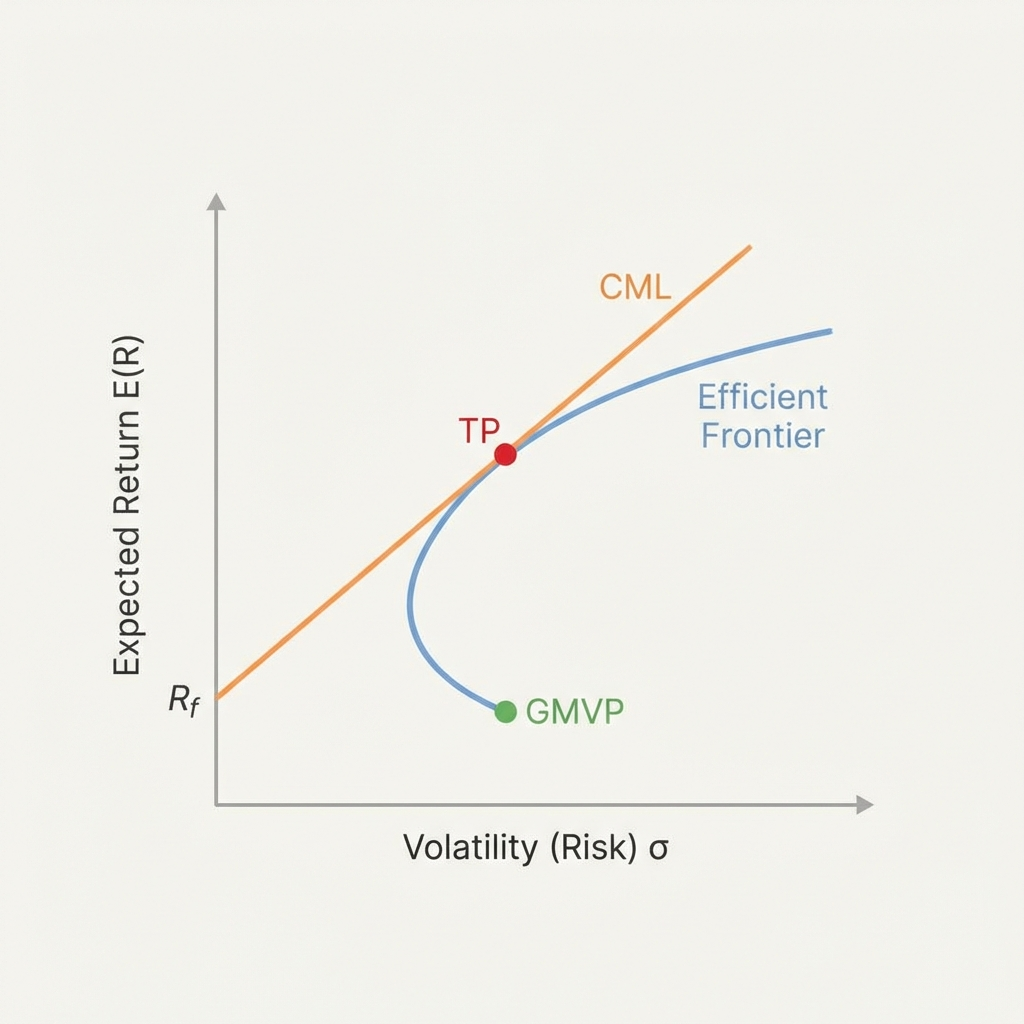
\includegraphics[width=0.8\textwidth]{efficient_frontier.png}
    \caption{Visualisasi Efficient Frontier dan Portofolio Optimal}
    \label{fig:frontier}
\end{figure}

\subsection{Portofolio yang Efisien}
Sebuah portofolio dikatakan efisien jika tidak ada portofolio lain yang:
\begin{itemize}
    \item Memiliki \textit{return} lebih tinggi dengan risiko yang sama.
    \item Memiliki risiko lebih rendah dengan \textit{return} yang sama.
\end{itemize}

\section{Minimum Variance Portfolio}
Titik paling kiri pada kurva \textit{Efficient Frontier} disebut sebagai \textit{Global Minimum Variance Portfolio} (GMVP). Portofolio ini adalah kombinasi aset yang menghasilkan risiko (varians) terendah dari seluruh kemungkinan kombinasi aset yang ada, tanpa mempedulikan berapa tingkat imbal hasil yang diperoleh. GMVP sangat penting bagi investor yang memiliki toleransi risiko sangat rendah namun tetap ingin mendiversifikasi investasinya.

\chapter{Matematika Optimalisasi Portofolio}

\section{Formulasi Masalah Optimalisasi}
Optimalisasi portofolio Markowitz secara matematis adalah masalah pemrograman kuadratik (*Quadratic Programming*). Fokusnya adalah menemukan bobot aset ($\mathbf{w}$) yang meminimalkan risiko (varians) untuk tingkat pengembalian tertentu.

\subsection{Fungsi Objektif}
Fungsi yang ingin kita minimalkan adalah varians portofolio ($\sigma_p^2$). Dalam notasi matriks, fungsi ini dinyatakan sebagai:
\begin{equation}
    f(\mathbf{w}) = \frac{1}{2} \mathbf{w}^T \mathbf{\Sigma} \mathbf{w}
\end{equation}
Di mana $\mathbf{\Sigma}$ adalah matriks kovarians yang bersifat \textit{positive semi-definite}. Penggunaan faktor $1/2$ bertujuan untuk menyederhanakan proses derivasi nantinya.

\subsection{Constraint (Batasan)}
Dalam model standar, terdapat dua batasan utama yang harus dipenuhi:
\begin{enumerate}
    \item \textbf{Budget Constraint:} Seluruh dana harus teralokasikan sepenuhnya ke dalam aset-aset yang dipilih.
    \begin{equation}
        \sum_{i=1}^{n} w_i = 1 \quad \text{atau} \quad \mathbf{w}^T \mathbf{1} = 1
    \end{equation}
    \item \textbf{Target Return Constraint:} Portofolio harus menghasilkan tingkat pengembalian yang diharapkan sesuai target investor ($\mu_p$).
    \begin{equation}
        \sum_{i=1}^{n} w_i E[R_i] = \mu_p \quad \text{atau} \quad \mathbf{w}^T \mathbf{\mu} = \mu_p
    \end{equation}
\end{enumerate}

\section{Optimalisasi dengan Dua Aset}
Kasus dua aset memberikan ilustrasi visual yang paling sederhana tentang bagaimana diversifikasi bekerja.

\subsection{Kasus Tanpa Short Selling}
Jika investor dilarang melakukan \textit{short selling}, maka terdapat batasan tambahan $0 \le w_i \le 1$. Solusi optimal biasanya berada di sepanjang kurva yang menghubungkan aset A dan aset B. Jika korelasi antar kedua aset rendah, kurva ini akan melengkung ke arah kiri (risiko rendah).

\subsection{Kasus dengan Short Selling}
\textit{Short selling} memungkinkan investor memiliki bobot negatif pada suatu aset (meminjam aset untuk dijual sekarang dan membelinya kembali nanti). Dengan \textit{short selling}, investor dapat mencapai titik-titik di luar rentang harga aset individual, yang terkadang memberikan peluang untuk mengurangi risiko lebih jauh lagi, namun dengan eksposur risiko teknis yang berbeda.

\section{Optimalisasi dengan N Aset}
Untuk portofolio dengan banyak aset ($n > 2$), perhitungan manual menjadi tidak mungkin dilakukan. Kita harus menggunakan aljabar linear dan komputasi numerik. Masalah ini tetap memiliki struktur yang sama: minimisasi fungsi kuadratik dengan batasan linear. Solusinya akan membentuk \textit{Efficient Frontier} yang merupakan permukaan hiperbola dalam ruang \textit{mean-variance}.

\section{Metode Lagrange Multiplier}
Metode ini adalah teknik kalkulus untuk menemukan nilai ekstrem (maksimum atau minimum) dari suatu fungsi yang disertai dengan beberapa batasan.

\subsection{Teori Lagrange Multiplier}
Diberikan fungsi tujuan $f(x)$ dan batasan $g(x) = c$. Kita membentuk fungsi baru yang disebut Lagrangian ($\mathcal{L}$):
\begin{equation}
    \mathcal{L}(x, \lambda) = f(x) - \lambda(g(x) - c)
\end{equation}
Di mana $\lambda$ adalah pengali Lagrange. Kondisi optimal dicapai ketika turunan parsial terhadap seluruh variabel sama dengan nol.

\subsection{Aplikasi pada Optimalisasi Portofolio}
Dalam optimalisasi Markowitz, kita memiliki dua batasan, sehingga kita menggunakan dua pengali Lagrange ($\lambda_1$ dan $\lambda_2$):
\begin{equation}
    \mathcal{L}(\mathbf{w}, \lambda_1, \lambda_2) = \frac{1}{2} \mathbf{w}^T \mathbf{\Sigma} \mathbf{w} - \lambda_1 (\mathbf{w}^T \mathbf{1} - 1) - \lambda_2 (\mathbf{w}^T \mathbf{\mu} - \mu_p)
\end{equation}
Dengan menurunkan fungsi Lagrangian ini terhadap $\mathbf{w}$, kita dapat menemukan sistem persamaan linear yang akan memberikan bobot optimal $w^*$ untuk setiap target \textit{return} $\mu_p$.

\chapter{Algoritma Markowitz}

\section{Representasi Matematis}
Untuk mengimplementasikan teori Markowitz ke dalam komputer, kita perlu mengubah persamaan-persamaan matematis ke dalam representasi matriks yang standar.

\subsection{Notasi Matriks}
Misalkan kita memiliki $n$ buah aset. Variabel-variabel utama direpresentasikan sebagai berikut:
\begin{itemize}
    \item $\mathbf{w} = [w_1, w_2, \dots, w_n]^T$ : Vektor kolom bobot portofolio.
    \item $\mathbf{\mu} = [E[R_1], E[R_2], \dots, E[R_n]]^T$ : Vektor kolom imbal hasil ekspektasi.
    \item $\mathbf{\Sigma} = \begin{bmatrix} \sigma_{11} & \dots & \sigma_{1n} \\ \vdots & \ddots & \vdots \\ \sigma_{n1} & \dots & \sigma_{nn} \end{bmatrix}$ : Matriks kovarians simetris ukuran $n \times n$.
\end{itemize}

\subsection{Formulasi Quadratic Programming}
Secara komputasional, masalah Markowitz sering diformulasikan dalam bentuk \textit{Quadratic Programming} (QP) standar:
\begin{equation}
    \min_{\mathbf{w}} \frac{1}{2} \mathbf{w}^T \mathbf{\Sigma} \mathbf{w}
\end{equation}
dengan batasan:
\begin{align}
    \mathbf{A}\mathbf{w} &= \mathbf{b} \\
    \mathbf{G}\mathbf{w} &\le \mathbf{h}
\end{align}
Di mana $\mathbf{A}$ dan $\mathbf{b}$ mewakili batasan kesamaan (\textit{equality constraints} seperti sum of weights = 1), sedangkan $\mathbf{G}$ dan $\mathbf{h}$ mewakili batasan ketidaksamaan (\textit{inequality constraints} seperti dilarang short selling).

\section{Langkah-Langkah Algoritma}
Algoritma untuk mendapatkan portofolio optimal mengikuti alur kerja sistematis berikut:

\subsection{Input Data}
Data input utama adalah harga penutupan historis aset dalam rentang waktu tertentu. Dari harga historis ini, kita menghitung \textit{log returns} atau \textit{simple returns}.

\subsection{Perhitungan Matriks Kovarians}
Langkah ini sangat krusial. Matriks kovarians $\mathbf{\Sigma}$ harus bersifat \textit{invertible} dan \textit{positive definite} agar proses optimalisasi stabil. Dalam prakteknya, sering kali digunakan teknik \textit{shrinkage} jika jumlah data historis terbatas dibandingkan jumlah aset.

\subsection{Proses Optimalisasi}
Komputer akan menggunakan algoritma numerik (seperti \textit{Interior-Point Method}) untuk mencari vektor $\mathbf{w}$ yang meminimalkan fungsi tujuan di bawah ruang solusi yang dibatasi oleh \textit{constraints}.

\subsection{Output: Bobot Optimal}
Hasil akhir adalah vektor bobot $\mathbf{w}^*$. Jika batasan $w_i \ge 0$ diterapkan, maka output akan berupa persentase alokasi yang tidak melibatkan peminjaman aset.

\section{Kasus Khusus}
Terdapat tiga jenis portofolio utama yang sering dicari menggunakan algoritma ini:

\subsection{Portofolio Minimum Variance}
Hanya meminimalkan $\mathbf{w}^T \mathbf{\Sigma} \mathbf{w}$ dengan batasan $\sum w_i = 1$, tanpa target \textit{return} tertentu. Ini adalah portofolio paling aman di \textit{Efficient Frontier}.

\subsection{Portofolio dengan Target Return}
Investor menentukan target imbal hasil tertentu (misalnya 10\% per tahun), dan algoritma mencari risiko terendah untuk mencapai target tersebut.

\subsection{Portofolio Tangent (Sharpe Optimal)}
Portofolio yang memiliki rasio imbal hasil terhadap risiko (\textit{Sharpe Ratio}) tertinggi. Secara geometris, ini adalah titik di mana garis dari \textit{risk-free rate} menyinggung kurva \textit{Efficient Frontier}.

\chapter{Implementasi Komputasional}

\section{Implementasi dengan Python}
Python telah menjadi bahasa standar dalam keuangan kuantitatif karena ekosistem pustakanya yang kaya dan mudah digunakan.

\subsection{Library yang Digunakan (NumPy, SciPy, pandas)}
Untuk membangun mesin optimalisasi Markowitz, kita membutuhkan tiga pustaka utama:
\begin{itemize}
    \item \textbf{Pandas:} Digunakan untuk manipulasi data deret waktu (*time-series*) dan membaca dataset harga saham.
    \item \textbf{NumPy:} Digunakan untuk operasi aljabar linear dan perhitungan matriks yang efisien.
    \item \textbf{SciPy (Optimize):} Menyediakan fungsi \texttt{minimize} yang mendukung pemrograman kuadratik dengan berbagai batasan.
\end{itemize}

\subsection{Contoh Kode Program}
Berikut adalah implementasi sederhana untuk mencari portofolio dengan varians minimum menggunakan \texttt{scipy.optimize}:

\begin{verbatim}
import numpy as np
import pandas as pd
from scipy.optimize import minimize

def get_portfolio_variance(weights, cov_matrix):
    return weights.T @ cov_matrix @ weights

# Data simulasi: Expected Return dan Matriks Kovarians
mu = np.array([0.1, 0.12, 0.15])
cov = np.array([[0.005, 0.002, 0.001],
                [0.002, 0.008, 0.003],
                [0.001, 0.003, 0.012]])

n_assets = len(mu)
init_weights = np.array([1/n_assets] * n_assets)

# Batasan: Jumlah bobot harus = 1
constraints = ({'type': 'eq', 'fun': lambda x: np.sum(x) - 1})
# Batasan: Tidak ada short selling (bobot 0 s/d 1)
bounds = tuple((0, 1) for asset in range(n_assets))

result = minimize(get_portfolio_variance, init_weights, 
                  args=(cov,), method='SLSQP', 
                  bounds=bounds, constraints=constraints)

print("Bobot Optimal:", result.x)
\end{verbatim}

\subsection{Visualisasi Efficient Frontier}
Visualisasi dilakukan dengan mensimulasikan ribuan kombinasi portofolio acak (*Monte Carlo Simulation*) atau dengan menyelesaikan masalah optimalisasi untuk berbagai target \textit{return}. Hasilnya diplot menggunakan \texttt{matplotlib} dengan sumbu x sebagai volatilitas (standar deviasi) dan sumbu y sebagai \textit{expected return}.

\section{Implementasi dengan R}
\subsection{Package yang Digunakan}
Dalam bahasa R, paket \texttt{PortfolioAnalytics} dan \texttt{quadprog} sering digunakan untuk keperluan ini. R sangat kuat dalam analisis statistik mendalam.

\subsection{Contoh Kode Program}
Contoh penggunaan \texttt{quadprog} di R:
\begin{verbatim}
library(quadprog)
# Setup Dmat (Kovarians), dvec, Amat, bvec sesuai spek QP
# solve.QP(Dmat, dvec, Amat, bvec)
\end{verbatim}

\section{Implementasi dengan MATLAB}
MATLAB menyediakan \texttt{Portfolio Object} dalam \textit{Financial Toolbox} yang sangat kuat. Pengguna cukup memasukkan data harga, dan MATLAB akan menghitung \textit{frontier} secara otomatis menggunakan fungsi \texttt{estimateFrontier}.

\section{Perbandingan Performa Komputasi}
Python unggul dalam integrasi dengan sistem produksi dan AI, sementara R unggul dalam visualisasi statistik. MATLAB tetap menjadi pilihan utama di lingkungan akademik dan institusi keuangan besar karena stabilitas dan dukungan teknisnya, meskipun bersifat berbayar.

\chapter{Capital Asset Pricing Model (CAPM)}

\section{Pengantar CAPM}
Capital Asset Pricing Model (CAPM) dikembangkan secara independen oleh Jack Treynor, William Sharpe \cite{sharpe1964capital}, John Lintner, dan Jan Mossin pada tahun 1960-an. Model ini merupakan pengembangan langsung dari Teori Portofolio Markowitz. Jika Markowitz memberikan kerangka kerja tentang cara membangun portofolio yang efisien bagi investor individu, CAPM melangkah lebih jauh dengan menjelaskan bagaimana harga aset ditentukan di pasar saat seluruh investor menggunakan prinsip Markowitz.

\section{Risk-Free Asset}
Salah satu kontribusi utama dalam pengembangan CAPM adalah pengenalan aset bebas risiko (*risk-free asset*). Aset bebas risiko adalah instrumen investasi yang memiliki varians nol (risikonya dianggap tidak ada), seperti obligasi pemerintah jangka pendek (misalnya T-bills di AS atau SUN di Indonesia). 
Dengan adanya aset bebas risiko, investor tidak hanya memilih kombinasi aset berisiko, tetapi juga dapat membagi dananya antara aset bebas risiko dan satu portofolio berisiko yang optimal.

\section{Capital Market Line (CML)}
Ketika aset bebas risiko tersedia, garis efisien yang tadinya berbentuk kurva hiperbola (Market Frontier) berubah menjadi garis lurus yang disebut \textit{Capital Market Line} (CML). Garis ini ditarik dari tingkat imbal hasil bebas risiko ($R_f$) dan menyinggung (\textit{tangent}) kurva \textit{Efficient Frontier} Markowitz. Seluruh investor yang rasional akan memilih kombinasi antara aset bebas risiko dan portofolio di titik singgung tersebut (lihat Gambar \ref{fig:frontier} pada Bab 4).

\section{Market Portfolio}
Titik singgung pada CML tersebut dikenal sebagai Portofolio Pasar (*Market Portfolio*). Dalam teori, portofolio ini berisi seluruh aset berisiko yang ada di pasar dengan bobot sesuai kapitalisasi pasarnya. CAPM menyimpulkan bahwa portofolio ini adalah portofolio aset berisiko yang paling efisien bagi semua investor, terlepas dari preferensi risiko mereka. Perbedaan antar investor hanya terletak pada seberapa besar proporsi dana yang mereka alokasikan pada aset bebas risiko dibandingkan pada portofolio pasar tersebut.

\section{Hubungan Markowitz dan CAPM}
Hubungan antara keduanya dapat diringkas sebagai berikut:
\begin{itemize}
    \item \textbf{Markowitz} memberikan metodologi untuk mengidentifikasi kumpulan portofolio efisien berdasarkan data historis.
    \item \textbf{CAPM} menggunakan hasil optimalisasi Markowitz untuk menurunkan model penetapan harga aset yang menghubungkan risiko sistematis ($\beta$) dengan imbal hasil yang diharapkan.
    \item Jika Markowitz berfokus pada risiko total (standar deviasi), CAPM menyatakan bahwa di pasar yang terdiversifikasi, investor hanya akan diberikan kompensasi atas risiko pasar (*systematic risk*) yang tidak dapat dihilangkan melalui diversifikasi.
\end{itemize}

\chapter{Pengembangan dan Modifikasi Model}

\section{Model Black-Litterman}
Model Black-Litterman, yang dikembangkan oleh Fischer Black dan Robert Litterman di Goldman Sachs pada tahun 1990 \cite{black1992global}, merupakan salah satu perbaikan paling populer terhadap model Markowitz. Masalah utama model Markowitz klasik adalah sensitivitasnya yang sangat tinggi terhadap input imbal hasil ekspektasi yang sering kali menghasilkan bobot portofolio yang tidak intuitif atau terkonsentrasi secara ekstrem.
Black-Litterman menggabungkan pandangan subjektif investor (*investor views*) dengan keseimbangan pasar (*market equilibrium*) menggunakan pendekatan Bayes. Hasilnya adalah portofolio yang lebih stabil dan terdiversifikasi dengan baik dibandingkan model Markowitz tradisional.

\section{Robust Portfolio Optimization}
Optimalisasi portofolio yang kokoh (*Robust Optimization*) menangani masalah ketidakpastian data input. Dalam Markowitz klasik, kita mengasumsikan bahwa \textit{mean} dan kovarians diketahui dengan pasti. Namun, dalam kenyataannya, parameter ini hanyalah estimasi yang mengandung error.
Pendekatan \textit{robust} membangun sebuah "himpunan ketidakpastian" (*uncertainty set*) untuk input tersebut dan mencari bobot portofolio yang memberikan performa terbaik dalam skenario terburuk (*worst-case scenario*).

\section{Risk Parity Portfolio}
Berbeda dengan Markowitz yang berfokus pada alokasi modal berdasarkan \textit{mean-variance}, \textit{Risk Parity} berfokus pada alokasi risiko. Tujuannya adalah memastikan bahwa setiap aset dalam portofolio memberikan kontribusi risiko yang sama besar. Strategi ini menjadi sangat populer setelah krisis keuangan 2008 karena dianggap lebih tangguh terhadap guncangan pada kelas aset tertentu (seperti ekuitas) yang biasanya mendominasi risiko portofolio tradisional.

\section{Conditional Value at Risk (CVaR)}
Salah satu kritik terbesar terhadap Markowitz adalah penggunaan varians sebagai proksi risiko, yang mengasumsikan distribusi keuntungan bersifat simetris. Namun, investor sebenarnya lebih peduli pada risiko kerugian ekstrem (*downside risk*).
*Conditional Value at Risk* (CVaR), atau dikenal juga sebagai *Expected Shortfall* \cite{rockafellar2000optimization}, mengukur rata-rata kerugian pada ekor distribusi (misalnya 5\% terburuk). Optimalisasi berbasis CVaR sangat berguna untuk aset yang memiliki distribusi tidak normal dengan ekor yang gemuk (*fat tails*), seperti mata uang kripto.

\section{Mean-Absolute Deviation Model}
Model *Mean-Absolute Deviation* (MAD), yang diperkenalkan oleh Konno dan Yamazaki pada tahun 1991 \cite{konno1991mean}, merupakan alternatif yang lebih efisien secara komputasi dibandingkan model varians kuadratik. Dengan menggunakan deviasi absolut rata-rata sebagai ukuran risiko, masalah optimalisasi berubah dari pemrograman kuadratik menjadi pemrograman linear (*Linear Programming*), yang jauh lebih mudah dan cepat diselesaikan untuk portofolio dengan ribuan aset.

\chapter{Studi Kasus dan Aplikasi Praktis}

\section{Studi Kasus: Portofolio Saham Indonesia}
Dalam bagian ini, kita akan menerapkan algoritma Markowitz pada data nyata dari Bursa Efek Indonesia (BEI). Misalkan kita memilih 5 saham dari indeks LQ45 (seperti BBCA, ASII, TLKM, UNVR, dan GOTO) untuk periode pengamatan satu tahun terakhir.

\subsection{Pemilihan Saham}
Saham yang dipilih mewakili berbagai sektor (perbankan, otomotif, telekomunikasi, konsumsi, dan teknologi) untuk memaksimalkan potensi manfaat diversifikasi melalui korelasi yang rendah antar sektor.

\begin{table}[h]
    \centering
    \caption{Data Statistik Historis Saham Pilihan (Estimasi)}
    \label{tab:saham_stats}
    \begin{tabular}{|c|c|c|c|}
        \hline
        \textbf{Ticker} & \textbf{Sektor} & \textbf{Avg Return (Harian)} & \textbf{Std Dev (Risiko)} \\ \hline
        BBCA & Perbankan & 0.05\% & 1.1\% \\ \hline
        ASII & Otomotif & 0.02\% & 1.8\% \\ \hline
        TLKM & Telekomunikasi & 0.03\% & 1.5\% \\ \hline
        UNVR & Konsumsi & -0.01\% & 1.4\% \\ \hline
        GOTO & Teknologi & 0.10\% & 3.5\% \\ \hline
    \end{tabular}
\end{table}

\subsection{Pengumpulan Data}
Data harga penutupan harian diperoleh dari penyedia data seperti Yahoo Finance atau RTI Business. Harga-harga ini kemudian diubah menjadi \textit{log returns} untuk memastikan sifat aditif dari waktu ke waktu.

\subsection{Analisis dan Optimalisasi}
Setelah menghitung vektor \textit{mean return} harian dan matriks kovarians, kita menjalankan proses optimalisasi. Hasilnya menunjukkan bahwa untuk tingkat risiko tertentu, alokasi mungkin akan lebih berat pada BBCA karena stabilitas volatilitasnya yang historis, sementara saham dengan volatilitas tinggi seperti GOTO mungkin akan memiliki bobot yang sangat rendah jika investor memiliki profil risiko moderat.

\subsection{Backtesting}
\textit{Backtesting} dilakukan dengan menerapkan bobot optimal yang dihitung pada periode T, lalu mengamati kinerjanya pada periode T+1. Kita membandingkan kinerja portofolio Markowitz ini terhadap indeks acuan (IHSG). Hasil \textit{backtesting} sering kali menunjukkan bahwa meskipun portofolio Markowitz memiliki volatilitas yang lebih rendah, performanya sangat bergantung pada apakah kondisi pasar di masa depan konsisten dengan data historis yang digunakan.

\section{Studi Kasus: Portofolio Multi-Asset}
Aplikasi Markowitz tidak terbatas pada saham. Seorang investor institusi mungkin mengombinasikan saham, obligasi pemerintah (ORI/FR), emas, dan reksadana pasar uang. Diversifikasi antar kelas aset (\textit{Asset Allocation}) terbukti jauh lebih efektif dalam mengurangi risiko sistematis dibandingkan hanya diversifikasi antar saham dalam satu negara.

\section{Analisis Sensitivitas}
Analisis sensitivitas dilakukan untuk melihat seberapa jauh perubahan kecil pada estimasi imbal hasil atau korelasi akan mengubah bobot portofolio. Kita akan menemukan bahwa model Markowitz sangat sensitif terhadap perubahan kecil pada \textit{expected return}, yang menguatkan argumen perlunya penggunaan model seperti Black-Litterman atau teknik \textit{shrinkage}.

\section{Rebalancing Portofolio}
Kondisi pasar selalu berubah, menyebabkan bobot aset dalam portofolio bergeser dari proporsi optimalnya seiring waktu. \textit{Rebalancing} adalah proses menyesuaikan kembali bobot aset ke target optimal secara berkala (misalnya setiap kuartal atau semester). Hal ini penting untuk menjaga profil risiko investasi agar tetap sesuai dengan rencana awal.

\chapter{Kritik dan Keterbatasan}

Meskipun Teori Portofolio Markowitz merupakan fondasi bagi keuangan modern, dalam aplikasinya terdapat berbagai kritik dan keterbatasan yang perlu dipahami oleh para praktisi.

\section{Asumsi yang Tidak Realistis}
Banyak asumsi dasar Markowitz yang dianggap terlalu menyederhanakan realitas pasar keuangan yang kompleks.

\subsection{Distribusi Normal Return}
Markowitz mengasumsikan bahwa *return* aset mengikuti distribusi normal. Namun, data historis menunjukkan bahwa pasar keuangan sering kali mengalami fenomena *fat tails* (ekor gemuk), di mana kejadian ekstrem (seperti krisis keuangan) terjadi lebih sering daripada yang diprediksi oleh distribusi normal. Penggunaan varians sebagai ukuran risiko tunggal gagal menangkap risiko asimetris dan kerugian ekstrem ini.

\subsection{Stabilitas Parameter}
Model ini mengasumsikan bahwa nilai rata-rata (*mean*) dan matriks kovarians bersifat statis atau stabil dari waktu ke waktu. Kenyataannya, korelasi antar aset cenderung meningkat secara drastis saat terjadi krisis pasar (*correlation breakdown*), sehingga manfaat diversifikasi yang diharapkan justru menghilang tepat saat paling dibutuhkan.

\section{Estimation Error}
Masalah terbesar dalam implementasi praktis adalah "sensitivitas input". Kesalahan kecil dalam mengestimasi *expected return* dapat mengakibatkan perubahan drastis pada bobot portofolio optimal. Hal ini sering membuat portofolio Markowitz menjadi "mesin peningkat kesalahan" (*error maximizer*), di mana model justru memberikan bobot besar pada aset yang imbal hasilnya diestimasi terlalu tinggi atau risikonya diestimasi terlalu rendah karena data historis yang kurang representatif.

\section{Transaction Costs dan Taxes}
Model Markowitz standar mengabaikan adanya biaya transaksi (komisi broker, *spread* harga) dan pajak. Dalam dunia nyata, melakukan penyesuaian bobot (*rebalancing*) secara terus-menerus mengikuti titik optimal dapat memakan biaya yang sangat besar, yang jika tidak diperhitungkan, dapat menghapus seluruh keuntungan tambahan yang diperoleh dari optimalisasi tersebut.

\section{Masalah Implementasi Praktis}
Sering kali, optimalisasi Markowitz menghasilkan portofolio yang terkonsentrasi hanya pada segelintir aset (bobot ekstrem 0 atau 1), yang secara psikologis sulit diterima oleh investor. Selain itu, model ini tidak memperhitungkan likuiditas; sebuah aset mungkin terlihat optimal secara matematis, tetapi dalam jumlah besar, aset tersebut tidak dapat dibeli atau dijual dengan cepat tanpa menggerakkan harga pasar.

\chapter{Perkembangan Terkini}

Dunia investasi terus berevolusi seiring dengan kemajuan teknologi dan perubahan prioritas global. Teori Markowitz yang telah berusia lebih dari tujuh dekade kini diadaptasi untuk menjawab tantangan zaman baru.

\section{Machine Learning dalam Optimalisasi Portofolio}
Kemunculan \textit{Machine Learning} (ML) membawa perubahan besar dalam cara investor mengestimasi input untuk model Markowitz. Algoritma seperti \textit{Random Forest}, \textit{Long Short-Term Memory} (LSTM), dan \textit{Reinforcement Learning} digunakan untuk memprediksi \textit{expected return} dan matriks kovarians dengan lebih akurat dibandingkan metode statistik tradisional. Selain itu, ML mampu menangani data non-linear dan hubungan antar aset yang kompleks yang tidak tertangkap oleh model linear klasik.

\section{ESG (Environmental, Social, Governance) dalam Portofolio}
Saat ini, investor tidak hanya mengejar imbal hasil finansial, tetapi juga dampak sosial dan lingkungan. Integrasi skor ESG ke dalam optimalisasi Markowitz dilakukan dengan menambahkan batasan (*constraint*) tambahan pada fungsi tujuan. Misalnya, investor dapat menetapkan target nilai ESG minimum untuk keseluruhan portofolio, sehingga algoritma akan memilih kombinasi aset yang efisien secara finansial sekaligus bertanggung jawab secara sosial.

\section{High-Frequency Trading dan Markowitz}
Di era \textit{High-Frequency Trading} (HFT), optimalisasi portofolio tidak lagi dilakukan secara bulanan atau harian, melainkan dalam hitungan milidetik. Algoritma Markowitz diadaptasi untuk bekerja pada frekuensi tinggi dengan memperhitungkan mikrostruktur pasar dan biaya dampak perdagangan (*market impact cost*). Kecepatan eksekusi dan efisiensi algoritma menjadi faktor penentu keberhasilan dalam lingkungan ini.

\section{Cryptocurrency Portfolio Optimization}
Mata uang kripto (*Cryptocurrency*) telah menjadi kelas aset baru yang menarik minat investor institusi. Karakteristik kripto yang memiliki volatilitas sangat tinggi dan korelasi yang rendah dengan aset tradisional (seperti saham dan emas) menjadikannya kandidat menarik untuk diversifikasi. Namun, karena distribusinya yang sering kali memiliki \textit{extreme fat tails}, optimalisasi portofolio kripto sering kali menggunakan modifikasi Markowitz seperti model CVaR atau optimalisasi berbasis entropi untuk mengelola risiko kerugian ekstrem.

\chapter{Penutup}

\section{Ringkasan}
Buku ini telah menelusuri perjalanan panjang Teori Portofolio Markowitz, mulai dari konsep dasar *risk* dan *return* hingga implementasi algoritma yang kompleks di era digital. Kita telah mempelajari bahwa inti dari kontribusi Markowitz bukan hanya pada pemilihan aset individual, melainkan pada pemahaman tentang bagaimana aset-aset tersebut berinteraksi dalam sebuah kesatuan portofolio. Melalui diversifikasi yang cerdas dan optimalisasi matematis, investor dapat mencapai efisiensi yang tidak mungkin didapatkan dengan hanya mengandalkan intuisi.

\section{Arah Penelitian Masa Depan}
Meskipun sudah berusia lebih dari 70 tahun, bidang optimalisasi portofolio masih terus berkembang. Fokus penelitian di masa depan kemungkinan besar akan berpusat pada:
\begin{itemize}
    \item \textbf{Explainable AI (XAI):} Mengembangkan model machine learning yang tidak hanya akurat dalam memprediksi *return*, tetapi juga dapat dijelaskan logika di balik alokasi asetnya.
    \item \textbf{Optimalisasi Dinamis:} Menangani masalah optimalisasi dalam waktu kontinu dengan mempertimbangkan biaya transaksi yang dinamis.
    \item \textbf{Integrasi Big Data:} Memanfaatkan data alternatif seperti sentimen media sosial dan gambar satelit secara langsung ke dalam kerangka kerja Markowitz untuk mendapatkan keunggulan informasi (*informational edge*).
\end{itemize}

\section{Kesimpulan}
Teori Portofolio Markowitz tetap menjadi kerangka kerja paling berpengaruh dalam dunia investasi. Meskipun memiliki keterbatasan dan asumsi yang sering kali tidak realistis, prinsip dasarnya mengenai efisiensi dan diversifikasi tetap relevan dan tak tergantikan. Bagi para akademisi dan praktisi, memahami Markowitz adalah langkah pertama yang krusial sebelum melangkah ke model keuangan yang lebih maju. Sebagaimana pepatah dalam dunia keuangan, "Diversifikasi adalah satu-satunya makan siang gratis di pasar modal," dan Markowitz adalah orang yang memberikan kita resep untuk menyajikannya.

\appendix

\chapter{Tinjauan Aljabar Linear}
Bagian ini memberikan tinjauan singkat mengenai konsep aljabar linear yang digunakan dalam buku ini.

\section{Vektor dan Matriks}
Vektor adalah susunan angka dalam satu kolom atau baris. Dalam konteks portofolio, kita sering menggunakan vektor bobot $\mathbf{w}$ dan vektor imbal hasil $\mathbf{\mu}$. Matriks $\mathbf{\Sigma}$ adalah kumpulan angka yang disusun dalam baris dan kolom, yang dalam buku ini digunakan untuk mewakili kovarians antar aset.

\section{Operasi Matriks}
Operasi yang paling sering digunakan adalah perkalian matriks. Misalnya, varians portofolio dihitung sebagai $\mathbf{w}^T \mathbf{\Sigma} \mathbf{w}$. Ini melibatkan operasi transposisi ($\mathbf{w}^T$) dan perkalian titik antar elemen.

\section{Invers Matriks}
Invers dari matriks $\mathbf{\Sigma}$, yang dilambangkan dengan $\mathbf{\Sigma}^{-1}$, digunakan untuk mencari solusi analitis dari bobot portofolio ketika menggunakan metode Lagrange Multiplier. Hanya matriks persegi yang non-singular (determinan $\neq 0$) yang memiliki invers.

\section{Eigen Values dan Eigen Vectors}
Nilai eigen dan vektor eigen sangat penting untuk memahami sifat matriks kovarians. Matriks kovarians yang valid harus bersifat *positive semi-definite*, yang berarti seluruh nilai eigennya harus lebih besar atau sama dengan nol.

\chapter{Tinjauan Kalkulus}
Optimalisasi Markowitz didasarkan pada teknik kalkulus peubah banyak.

\section{Turunan Parsial}
Turunan parsial digunakan untuk menemukan gradien dari fungsi tujuan (varians) dan fungsi batasan. Nilai optimal ditemukan ketika gradien dari Lagrangian sama dengan nol.

\section{Optimalisasi Tanpa Batasan}
Dalam kasus sederhana tanpa batasan, titik minimum ditemukan dengan menetapkan turunan pertama sama dengan nol dan memastikan turunan kedua bernilai positif.

\section{Optimalisasi dengan Batasan}
Metode Lagrange Multiplier, sebagaimana dibahas di Bab 5, adalah cara standar untuk menangani batasan kesamaan dalam masalah optimalisasi. Untuk batasan ketidaksamaan (seperti $w_i \ge 0$), kita menggunakan syarat Karush-Kuhn-Tucker (KKT).

\chapter{Tabel Distribusi Statistik}
Lampiran ini biasanya berisi tabel z untuk distribusi normal standar, yang digunakan untuk menghitung probabilitas jika variabel mengikuti distribusi normal. Dalam era digital, nilai-nilai ini umumnya dihitung langsung menggunakan perangkat lunak seperti Excel atau pustaka Python `scipy.stats`.

\chapter{Dataset untuk Latihan}
Dataset yang digunakan dalam contoh buku ini dapat diakses secara daring atau direkonstruksi menggunakan API keuangan. Dataset mencakup:
\begin{itemize}
    \item Harga penutupan harian 5 saham Blue Chip BEI (2023-2024).
    \item Data obligasi pemerintah tenor 10 tahun sebagai *proxy* aset bebas risiko.
    \item Data harga harian Emas (Antam) sebagai instrumen diversifikasi.
\end{itemize}

\backmatter

\bibliographystyle{plain}
\bibliography{references}

\printindex

\end{document}
